\tikzset{every picture/.style={line width=0.75pt}} %set default line width to 0.75pt        

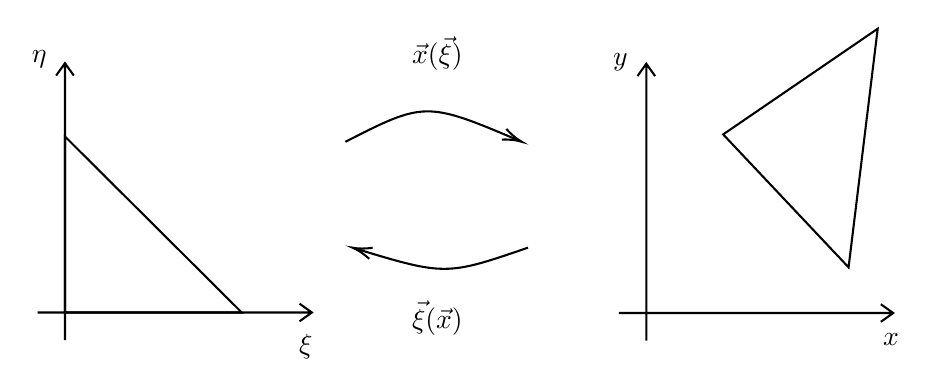
\begin{tikzpicture}[x=0.75pt,y=0.75pt,yscale=-0.85,xscale=0.85]
%uncomment if require: \path (0,300); %set diagram left start at 0, and has height of 300
%Shape: Triangle [id:dp7899633980320873] 
\draw   (90.05,130.5) -- (190.25,230.25) -- (90.05,230.25) -- cycle ;
%Shape: Axis 2D [id:dp4410284844713135] 
\draw  (74.5,230.25) -- (230,230.25)(90.05,88.95) -- (90.05,245.95) (223,225.25) -- (230,230.25) -- (223,235.25) (85.05,95.95) -- (90.05,88.95) -- (95.05,95.95)  ;
%Curve Lines [id:da26067351400473004] 
\draw    (249,133.5) .. controls (293.55,110.73) and (294.98,110.5) .. (347.4,132.82) ;
\draw [shift={(349,133.5)}, rotate = 203.07] [color={rgb, 255:red, 0; green, 0; blue, 0 }  ][line width=0.75]    (10.93,-3.29) .. controls (6.95,-1.4) and (3.31,-0.3) .. (0,0) .. controls (3.31,0.3) and (6.95,1.4) .. (10.93,3.29)   ;
%Shape: Triangle [id:dp8761891095630314] 
\draw   (550.72,69.4) -- (534.21,204.66) -- (463.13,129.31) -- cycle ;
%Shape: Axis 2D [id:dp4074126648350844] 
\draw  (404,230.55) -- (559.5,230.55)(419.55,89.25) -- (419.55,246.25) (552.5,225.55) -- (559.5,230.55) -- (552.5,235.55) (414.55,96.25) -- (419.55,89.25) -- (424.55,96.25)  ;
%Curve Lines [id:da2988864034647969] 
\draw    (352.5,193.5) .. controls (306.46,209.34) and (305.51,209.5) .. (254.56,193.98) ;
\draw [shift={(253,193.5)}, rotate = 16.95] [color={rgb, 255:red, 0; green, 0; blue, 0 }  ][line width=0.75]    (10.93,-3.29) .. controls (6.95,-1.4) and (3.31,-0.3) .. (0,0) .. controls (3.31,0.3) and (6.95,1.4) .. (10.93,3.29)   ;

% Text Node
\draw (221,241) node [anchor=north west][inner sep=0.75pt]   [align=left] {$\xi$};
% Text Node
\draw (69.5,80) node [anchor=north west][inner sep=0.75pt]   [align=left] {$\eta $};
% Text Node
\draw (552,240.5) node [anchor=north west][inner sep=0.75pt]   [align=left] {$x$};
% Text Node
\draw (399,81.5) node [anchor=north west][inner sep=0.75pt]   [align=left] {$y$};
% Text Node
\draw (285,72) node [anchor=north west][inner sep=0.75pt]   [align=left] {$\vec{x}(\vec{\xi})$};
% Text Node
\draw (285,222) node [anchor=north west][inner sep=0.75pt]   [align=left] {$\vec{\xi}(\vec{x})$};


\end{tikzpicture}
